%% Springer Nature LaTeX template (sn-jnl), Math and Physical Sciences numbered reference style
\documentclass[pdflatex,sn-mathphys-num]{sn-jnl}

\usepackage{graphicx}%
\usepackage{multirow}%
\usepackage{amsmath,amssymb,amsfonts}%
\usepackage{amsthm}%
\usepackage{mathrsfs}%
\usepackage[title]{appendix}%
\usepackage{xcolor}%
\usepackage{textcomp}%
\usepackage{manyfoot}%
\usepackage{booktabs}%
\usepackage{algorithm}%
\usepackage{algorithmicx}%
\usepackage{algpseudocode}%
\usepackage{listings}%
\usepackage{array}%
\usepackage{rotating}%

\raggedbottom

\begin{document}

\title[Calibrated Three-Way Gating of Multimodal Auto-Insurance Claims]{Calibrated Three-Way Gating of Multimodal Auto-Insurance Claims with a Closed-Set Decision Model}

%% TODO(authors): confirm the first author's e-mail (the original author list wrote it with a space).
\author*[1]{\fnm{Kadiyala} \sur{Rajesh}}\email{rajesh\_kadiyala@srmap.edu.in}

\author[1]{\fnm{Matta} \sur{Vikas}}\email{matta\_vikas@srmap.edu.in}

\author[1]{\fnm{Mudigonda} \sur{Krishna Siva Prasad}}\email{krishna\_siva\_prasad@srmap.edu.in}

\affil*[1]{\orgdiv{Department of Computer Science and Engineering}, \orgname{SRM AP University}, \orgaddress{\city{Amaravati}, \postcode{522240}, \country{India}}}

%% Abstract is written last, after Results and Discussion (course guideline).
\abstract{Motor insurers must route each claim to automatic settlement, fraud audit or human review, using a damage photograph, a description and policy fields. Recent systems treat images and claim records separately, produce binary outputs, and leave the per-decision cost of language models unmeasured. We route claims with Gemini Decision 1, a closed-set model that answers a routing question and four yes/no checks over all three inputs in one request; a 24-parameter combiner and cost-aware gate escalate uncertain claims. We evaluate on a constructed, rule-labelled 1,000-claim benchmark pairing CarDD photographs with Auto Insurance Claims records. The router reaches 0.866 accuracy in repeated cross-validation and 0.853 on the frozen test split, against 0.908 and 0.913 for trained early fusion. At moderate cost weights it lowers misrouting cost against escalating every claim by 0.246, but not once every human review is charged. With 25 labels it reaches 0.825, against 0.754 for a rule-aware learner and 0.609 for early fusion. Its answers beat a generative model's answers to the same questions by 5.2 accuracy points, at 5--8 times lower latency and 6.5--18 times lower cost. Much of the small-sample lead comes from questions written from the labelling rules, which every method partly exploits.}


\keywords{insurance claim triage, multimodal fusion, selective prediction, calibration, human-in-the-loop, decision model}

\maketitle

\section{Introduction}\label{sec:intro}

Motor insurers handle claims in large numbers, and much of the cost lies in manual assessment: surveyors inspect photographs, read the claimant's account and check the policy record, and different assessors often reach different conclusions about the same case~\cite{ouf2026,cheng2026}. Insurers therefore automate digital first notice of loss, image-based damage detection, repair-cost estimation and fraud screening~\cite{arconzo2026,subhash2026,ouf2026}; in one deployment, conversational agents with damage detection cut processing time from 30 to 12 minutes~\cite{arconzo2026}. The risks are asymmetric. Approving a fraudulent claim loses money, auditing a legitimate one delays payment and adds handling cost, and a small, imbalanced fraud class makes the trade-off harder to control~\cite{bekkaye2026}. Deciding which claims to settle automatically, which to audit and which to give to a person is a practical problem worth studying.

This paper studies that routing decision, which we call \emph{claim gating}. Each claim has a photograph of the damaged vehicle, a short categorical description and eleven numerical fields, and the system assigns \emph{Auto-Approve}, \emph{Reject/Fraud-Audit} or \emph{Escalate-Human}. The task is hard because the photograph may show more or less damage than reported or be blurred, dark or cropped, the description may be incomplete, and errors carry different costs. We study it offline on a constructed 1,000-claim benchmark pairing CarDD photographs~\cite{wang2023cardd} with unrelated records from a public claims data set~\cite{kaggleclaims}; its labels follow documented construction rules, so results describe routing under those rules, not on real claims. Repair-cost estimation and forgery detection are out of scope.

The 2026 studies we surveyed leave four gaps. First, damage assessment and fraud prediction are studied separately~\cite{subhash2026}: vision models judge the photograph alone~\cite{ouf2026,li2026part,dalal2026,cheng2026}, and fraud models score the claim table without it~\cite{bekkaye2026,ebinezer2026,vandervorst2026}. Second, outputs are mostly binary; routing uncertain cases to people has been developed for payment and healthcare fraud~\cite{liu2026daunt,sourav2026,dadi2026,syed2026}, not for motor claims with photographs. Third, calibration and expected cost have been analysed for tabular motor-fraud models~\cite{bekkaye2026} and abstention for image-only damage assessment~\cite{shao2026}, but no study checks whether the photograph agrees with the claimed severity before deciding. Fourth, motor-claim systems that use language models generate text inside multi-stage pipelines~\cite{arconzo2026,mitrenga2026,phuengpanyaloet2026,hatzesberger2026}; none reports the per-call latency and cost of a routing decision or compares a closed-set decision model with a generative model asked the same questions, although per-path latency has been reported for transaction fraud~\cite{sourav2026}. What is missing is a calibrated, cost-aware, three-way routing policy that uses all three kinds of evidence and checks them against one another.

We build such a router on Gemini Decision~1, a hosted multimodal model that scores closed-set questions in one forward pass and returns option probabilities instead of text~\cite{google2026decisions}. One request carries the photograph, the description and the numbers as labelled text, and asks a three-option routing question and four yes/no checks: whether the visible damage matches the reported severity, whether the photograph is clear, whether the details are complete, and whether the amounts match the severity. Two checks compare modalities directly (image with text, numbers with text). Because the model generates no text and has a lower list price, a decision may be cheaper and faster than a generative one; we measure this against a generative model given the same questions, resolution and combiner, which compares two hosted products rather than two mechanisms.

A 24-parameter logistic combiner maps the answers to route probabilities, and a claim is approved or audited automatically only when the routing confidence clears a threshold chosen on validation to minimise a misrouting cost in which a wrong approval is the most expensive error; otherwise it is escalated, following the reject option~\cite{chow1970} and selective classification~\cite{geifman2017selective}. We assess accuracy, calibration~\cite{guo2017calibration,naeini2015,brier1950}, risk--coverage, misrouting and handling cost, latency and cost, on a fixed split and in repeated cross-validation, against single-modality, trained-fusion and generative baselines, with the same shortcut controls for every method.

The contributions of this paper are as follows.
\begin{itemize}
\item \textbf{A documented tri-modal claim-gating benchmark.} It contains 1,000 claim--photograph pairs with an image, a description, eleven numerical fields, three routing labels and a fixed split. We document its construction rules and measure the shortcuts they create; the record set will be released subject to the terms of both source data sets, and the images remain subject to the CarDD licence.
\item \textbf{A cost-aware three-way gating formulation.} Claim gating is formalised as selective three-way classification with an escalation class and an asymmetric cost matrix. At moderate cost weights the gate lowers misrouting cost against escalating every claim in cross-validation; once every human review is charged, it is no better than escalating everything.
\item \textbf{A single-request closed-set decision design.} Five questions, including image--text and number--text consistency checks, are answered in one request and combined by 24 parameters. The answers are more accurate routing features than a generative model's answers to the same questions, and, because the questions were written from the routing rules, few labels are needed: with 25 labelled claims the router reaches 0.825 accuracy, against 0.754 for a learner given the rules as features and 0.609 for trained fusion.
\item \textbf{An evaluation protocol with released code and cached responses.} The configuration was frozen before it was scored on test, and the router is compared with text, numerical, image, early-fusion, generative and rule-aware baselines using exact tests, corrected cross-validation tests, learning curves, a stability re-test, a photograph-degradation control and ablations. The benchmark build files were not kept, so the benchmark cannot be rebuilt from the source data sets.
\end{itemize}

\section{Literature Review}\label{sec:litreview}

We review peer-reviewed work published in 2026, found through three structured searches of a scholarly index and checked against Crossref and OpenAlex, plus classic method papers; gap statements refer to this surveyed literature. Table~\ref{tab:lit} compares the closest studies.

\paragraph{Single-modality claim analytics.}
Tabular fraud models show that calibration and cost can be measured: for motor fraud, Bekkaye et al.~\cite{bekkaye2026} found CatBoost the most balanced classifier and TabNet the lowest expected cost. Related work adds interpretability~\cite{ebinezer2026}, graph-aware boosting~\cite{vandervorst2026}, human-in-the-loop audit prioritisation~\cite{huang2026} and serialisation of numbers into text for small language models~\cite{slm2026}, which supports our numerical input format. None sees the photograph. Vision models estimate damage type, location and severity~\cite{ouf2026,li2026part,dalal2026}, reaching 89.30\% accuracy at about 6\,ms per image on CarDD~\cite{wang2023cardd,cheng2026}, but they answer \emph{what damage is visible}, not \emph{whether the claim is believable}, and area-based severity depends on viewpoint~\cite{li2026part}. Shao et al.~\cite{shao2026} added abstention and coverage--risk analysis to vision--language damage assessment, on images alone.

\paragraph{Multimodal fraud and claim systems.}
In motor claims, damage detection and fraud prediction have developed separately; one system passes detector descriptors to a random forest~\cite{subhash2026}, and FADES~\cite{arconzo2026} combines language-model agents, detectors trained on 13,353 accident images and rule-based severity, but reports a large domain gap on CarDD. Elsewhere, tri-modal fusion is learned end to end~\cite{nazir2026,ping2026,tatavarthi2026}: trust in each modality is buried in learned weights, the output is a fraud score rather than a route, and learned fusion degrades on noisy or low-quality inputs~\cite{zhang2026fusion}. T-CAMIF~\cite{akhtar2026} instead makes text--image inconsistency an explicit, informative feature, an idea not yet applied to a claim and its photograph.

\paragraph{Language models, deferral and calibration.}
Language models extract features from actuarial text and accident narratives~\cite{hatzesberger2026,hao2026traffic,chen2026bus}, generate forms and damage descriptions~\cite{arconzo2026,phuengpanyaloet2026}, or classify damage when prompted~\cite{mitrenga2026}; none of these studies reports the latency or cost of a model decision or uses a model that returns probabilities over fixed options. Withholding a decision dates to Chow's reject rule~\cite{chow1970} and selective classification~\cite{geifman2017selective}. Fraud systems defer transactions on which an ensemble disagrees, raising recall from 0.76 to 0.91 at 5\% deferral~\cite{liu2026daunt}, escalate cases whose rationales fail a verifier~\cite{sourav2026}, or route low-confidence cases to people~\cite{syed2026,dadi2026}; surveys treat abstention as the central hand-over mechanism~\cite{lazaros2026,punzi2026,presacan2026}. Reliability is reported with expected calibration error~\cite{naeini2015,guo2017calibration} and the Brier score~\cite{brier1950}. All of these deferral systems use tabular or transaction data.

\begin{sidewaystable}
\caption{Comparison of recent studies related to multimodal claim gating. Modalities: I = image, T = text, N = numerical/tabular, G = graph, L = document layout.}\label{tab:lit}
\scriptsize
\begin{tabular*}{\textheight}{@{\extracolsep{\fill}}>{\raggedright\arraybackslash}p{2.0cm}>{\raggedright\arraybackslash}p{2.3cm}>{\raggedright\arraybackslash}p{2.4cm}>{\raggedright\arraybackslash}p{1.0cm}>{\raggedright\arraybackslash}p{3.3cm}>{\raggedright\arraybackslash}p{2.9cm}>{\raggedright\arraybackslash}p{3.4cm}@{}}
\toprule
Reference & Problem/task & Data set & Modal. & Approach / fusion & Reported results & Limitations / relevance \\
\midrule
Bekkaye et al.~\cite{bekkaye2026} & Motor-insurance fraud & Auto-insurance fraud records & N & Six boosting and deep tabular models; resampling; calibration and expected cost & No single best model; TabNet lowest expected cost & No image or text; binary output \\
Ebinezer et al.~\cite{ebinezer2026} & Insurance fraud & 4,000 life claims, 83 attributes & N & CatBoost, Bi-GRU, TabTransformer; SHAP & Bi-GRU highest fraud recall & Tabular only; no deferral \\
El-Enen et al.~\cite{slm2026} & Medical-claim fraud & Medical activity records & T+N & Numbers and text serialised; small-LM embeddings; swarm feature selection & Up to 87\% accuracy & Supports text serialisation of numbers; no image \\
Cheng et al.~\cite{cheng2026} & Damage classification & CarDD and insurer data & I & Region-aware ResNet-50 mixture of experts & 89.30\% test accuracy; 6\,ms per image & Image only; same image source as ours \\
Li et al.~\cite{li2026part} & Part-level severity & Own damage set; public part set & I & YOLO11 segmentation; damage-to-part area ratio & Higher mAP at strict IoU & Area severity sensitive to viewpoint \\
Shao et al.~\cite{shao2026} & Vehicle damage state with abstention & 160 vehicles, 355 media & I & Two vision--language configurations; coverage--risk & Macro-F1 0.8645 vs 0.1923 & Abstention on images only \\
Arconzo et al.~\cite{arconzo2026} & First notice of loss and damage & 13,353 accident images & I+T+N & LLM agents; transformer detectors; rule-based severity & Processing 30$\rightarrow$12 min & Generative multi-stage; CarDD domain gap \\
Sri Subhash and Chellamani~\cite{subhash2026} & Motor claim verification & VehiDE and a constructed fraud set & I, N & Faster R-CNN descriptors fed to a random forest & 98\% accuracy; F1 0.85 & Sequential use of the image; binary \\
Nazir et al.~\cite{nazir2026} & Healthcare fraud & Healthcare claims & N+T+G & TabNet, ClinicalBERT, GAT; reliability-aware attention & 99.95\% accuracy reported & Near-perfect scores; opaque learned fusion \\
Ping et al.~\cite{ping2026} & Financial-statement fraud & 6,000+ EDGAR filings & N+T+L & Residual MLP, FinBERT, LayoutLMv2; gated fusion & AUC 0.923; F1 0.847 & Tri-modal fusion outside claims \\
Liu and Zhu~\cite{liu2026daunt} & Transaction fraud triage & ULB, IEEE-CIS & N & Ensemble disagreement; defer most uncertain & Recall 0.76$\rightarrow$0.91 at 5\% deferral & Deferral, but tabular only \\
Sourav et al.~\cite{sourav2026} & Financial fraud with verified rationales & Five public benchmarks & N+G & LightGBM triage; verified LM rationales; conformal calibration & p99 latency 10.23\,ms / 175.23\,ms & Escalation by verifier; no image \\
Akhtar and Rana~\cite{akhtar2026} & Text--image fake news & Twitter--Weibo & T+I & Cross-modal inconsistency features; trust-aware fusion & Accuracy 0.9061; AUC 0.9709 & Inconsistency as evidence, as in our check \\
\botrule
\end{tabular*}
\end{sidewaystable}

\paragraph{Research gap.}
No surveyed study decides on a motor claim from the photograph, description and numbers jointly, except through a multi-stage generative pipeline~\cite{arconzo2026}; calibrated deferral reaches motor claims only for image-only assessment~\cite{shao2026}; no motor-claim study uses claim--photograph agreement as an explicit decision signal~\cite{akhtar2026}; and the cost of a single model decision is unreported. Our method reads all three inputs in one request, turns cross-modal agreement into scores, gives a cost-aware three-way decision, and measures latency and cost against a generative model asked the same questions.

\section{Proposed Methodology}\label{sec:method}

The proposed method is a \emph{calibrated three-way claim gate}. It takes a vehicle photograph, a categorical claim description and eleven numerical claim and policy fields, and returns one of three routes: Auto-Approve ($\mathsf{A}$), Reject/Fraud-Audit ($\mathsf{R}$) or Escalate-Human ($\mathsf{E}$). Only $\mathsf{A}$ settles a claim without a person; $\mathsf{R}$ refers it to a human fraud investigation and never rejects it automatically (the name is the option text of the frozen routing question). The method has four stages: the numerical fields are serialised into a labelled text block; one request to Gemini Decision~1~\cite{google2026decisions} carries the photograph, the description, the numbers and five closed-set questions; a small learned combiner maps the returned probabilities to route probabilities; and a cost-aware threshold rule, tuned on the validation split, issues the route or escalates the claim. The inputs are fused twice: they are read jointly inside one request, and image--text and number--text agreement are asked as explicit questions. The decision model is used zero-shot. The only quantities fitted to data are the 24 combiner parameters and two thresholds.

\subsection{Mathematical model}\label{sec:math}

\paragraph{Inputs and scores.}
Let $\mathcal{D}=\{(x_i,y_i)\}_{i=1}^{N}$, $N=1{,}000$, be split into $\mathcal{D}_{\mathrm{tr}}$, $\mathcal{D}_{\mathrm{val}}$ and $\mathcal{D}_{\mathrm{te}}$. Each claim is
\begin{equation}
x_i=(I_i,\;T_i,\;\mathbf{n}_i),\qquad \mathbf{n}_i\in\mathbb{R}^{11},\qquad y_i\in\mathcal{Y}=\{\mathsf{A},\mathsf{R},\mathsf{E}\}, \label{eq:input}
\end{equation}
where $I_i$ is the JPEG photograph, $T_i$ the categorical description, $\mathbf{n}_i$ the eleven numerical fields and $y_i$ the routing label. Escalation is a valid class: a claim labelled $\mathsf{E}$ is handled correctly when it is escalated. A serialisation function $\phi:\mathbb{R}^{11}\rightarrow\Sigma^{*}$ writes the numbers as labelled text over the character set $\Sigma$, and the request is
\begin{equation}
r_i=\big\langle \iota,\; I_i,\; T_i,\; \phi(\mathbf{n}_i),\; \mathcal{Q}\big\rangle, \label{eq:request}
\end{equation}
with a fixed instruction $\iota$ and the questions $\mathcal{Q}=\{q_1,\dots,q_5\}$ of Table~\ref{tab:questions}. Question $q_j$ has options $\mathcal{O}_j$, with $\mathcal{O}_1=\mathcal{Y}$ and $\mathcal{O}_j=\{\textit{yes},\textit{no}\}$ for $j\ge2$. We treat the decision model as a black-box scorer $F$ that returns a distribution over each question's options,
\begin{equation}
\mathbf{p}_{ij}=F(r_i,q_j)\in\Delta^{|\mathcal{O}_j|-1},\qquad s_{ij}=p_{ij}(\textit{yes}),\quad j=2,\dots,5, \label{eq:scores}
\end{equation}
where $\Delta^{m}$ is the $m$-dimensional probability simplex. The service answers all questions about one input in a single forward pass and generates no output text~\cite{google2026decisions}; we do not assume its probabilities are calibrated. The checks mean, in order: the visible damage matches the reported severity ($s_{i2}$, image--text), the photograph is clear enough to judge ($s_{i3}$), the details are complete ($s_{i4}$), and the amounts match the reported severity ($s_{i5}$, number--text).

\paragraph{Learned combiner.}
A general decision model does not know a particular insurer's routing policy, so the seven probabilities form a feature vector
\begin{equation}
\mathbf{z}_i=\big(p_{i1}(\mathsf{A}),\,p_{i1}(\mathsf{R}),\,p_{i1}(\mathsf{E}),\,s_{i2},\,s_{i3},\,s_{i4},\,s_{i5}\big)\in[0,1]^{7}, \label{eq:features}
\end{equation}
mapped to route probabilities by a multinomial logistic regression,
\begin{equation}
h_y(\mathbf{z}_i)=\frac{\exp(\mathbf{w}_y^{\top}\mathbf{z}_i+b_y)}{\sum_{y'\in\mathcal{Y}}\exp(\mathbf{w}_{y'}^{\top}\mathbf{z}_i+b_{y'})},\qquad y\in\mathcal{Y}, \label{eq:combiner}
\end{equation}
with weights $\mathbf{w}_y\in\mathbb{R}^{7}$ and biases $b_y$ ($3\times8=24$ parameters $\boldsymbol{\Theta}$). They minimise the $L_2$-regularised cross-entropy on the training split,
\begin{equation}
\mathcal{L}_{\mathrm{comb}}(\boldsymbol{\Theta})=-\frac{1}{|\mathcal{D}_{\mathrm{tr}}|}\sum_{i\in\mathcal{D}_{\mathrm{tr}}}\log h_{y_i}(\mathbf{z}_i)+\frac{1}{2C\,|\mathcal{D}_{\mathrm{tr}}|}\sum_{y\in\mathcal{Y}}\lVert\mathbf{w}_y\rVert_2^2, \label{eq:combloss}
\end{equation}
where the inverse regularisation $C$ is selected from $\{0.01,0.1,1,10,100\}$ by validation log loss. The predicted route and its confidence are
\begin{equation}
\hat{y}_i=\arg\max_{y\in\mathcal{Y}}h_y(\mathbf{z}_i),\qquad c_i=\max_{y\in\mathcal{Y}}h_y(\mathbf{z}_i). \label{eq:route}
\end{equation}

\paragraph{Support and gate.}
An automatic approval should rest on consistent, clear and complete evidence, and an automatic audit on a clear photograph with at least one inconsistency:
\begin{equation}
\sigma_i(\mathsf{A})=\min\{s_{i2},s_{i3},s_{i4},s_{i5}\},\qquad \sigma_i(\mathsf{R})=\min\big\{s_{i3},\max\{1-s_{i2},1-s_{i5}\}\big\}, \label{eq:support}
\end{equation}
where $\min$ acts as a conjunction and $\max$ as a disjunction. For thresholds $\boldsymbol{\tau}=(\tau_c,\tau_s)\in[0,1]^2$ the gate issues
\begin{equation}
g_i(\boldsymbol{\tau})=
\begin{cases}
\hat{y}_i, & \text{if } \hat{y}_i\in\{\mathsf{A},\mathsf{R}\},\; c_i\ge\tau_c \text{ and } \sigma_i(\hat{y}_i)\ge\tau_s,\\
\mathsf{E}, & \text{otherwise;}
\end{cases} \label{eq:gate}
\end{equation}
$\tau_s=0$ gives a confidence-only gate.

\paragraph{Cost and objective.}
Routing errors have unequal consequences, so decisions are scored with
\begin{equation}
C(y,g)=\begin{cases}
0, & g=y,\\
c_{\mathrm{FA}},\ c_{\mathrm{FR}}\ \text{or}\ c_{\mathrm{H}}, & g=\mathsf{A},\ \mathsf{R}\ \text{or}\ \mathsf{E}\ \text{and}\ g\neq y,
\end{cases} \label{eq:cost}
\end{equation}
where $c_{\mathrm{FA}}$, $c_{\mathrm{FR}}$ and $c_{\mathrm{H}}$ are the costs of a wrongful approval, a wrongful audit and an unnecessary human review. We assume $c_{\mathrm{FA}}>c_{\mathrm{FR}}>c_{\mathrm{H}}>0$, use $(10,4,1)$ by default and test other values in Section~\ref{sec:exp}. With the combiner fixed, the thresholds minimise the empirical validation cost over the grid $\mathcal{T}=\{0,0.05,\dots,1\}^2$, with ties broken towards higher coverage:
\begin{equation}
\boldsymbol{\tau}^{*}=\arg\min_{\boldsymbol{\tau}\in\mathcal{T}}\;\frac{1}{|\mathcal{D}_{\mathrm{val}}|}\sum_{i\in\mathcal{D}_{\mathrm{val}}} C\big(y_i,\,g_i(\boldsymbol{\tau})\big). \label{eq:objective}
\end{equation}

\paragraph{Baselines and efficiency.}
Each supervised baseline outputs probabilities $\hat{\mathbf{p}}_i$ and minimises the cross-entropy $\mathcal{L}(\boldsymbol{\theta})=-\frac{1}{|\mathcal{D}_{\mathrm{tr}}|}\sum_{i\in\mathcal{D}_{\mathrm{tr}}}\log \hat{p}_i(y_i)$; it is gated by Eq.~(\ref{eq:gate}) with $c_i=\max_y\hat{p}_i(y)$, $\tau_s=0$ and $\tau_c$ from Eq.~(\ref{eq:objective}), so differences reflect the scores, not the decision rule. For each request we record the latency $\ell_i$ and billed tokens $u_i^{\mathrm{in}},u_i^{\mathrm{out}}$, and the cost per decision is
\begin{equation}
\kappa_i=\pi^{\mathrm{in}}u_i^{\mathrm{in}}+\pi^{\mathrm{out}}u_i^{\mathrm{out}}, \label{eq:apicost}
\end{equation}
with per-token prices $\pi^{\mathrm{in}},\pi^{\mathrm{out}}$ on the run date ($u_i^{\mathrm{out}}=0$ for Decision~1~\cite{google2026decisions}).

\subsection{Proposed architecture and algorithm}\label{sec:arch}

Figure~\ref{fig:architecture} shows the pipeline and Algorithm~\ref{alg:gate} lists its steps.

\begin{figure}[!htb]
\centering
%% Editable source: figures/architecture.drawio (draw.io); exported with draw.io CLI.
\includegraphics[width=\textwidth]{figures/architecture.png}
\caption{Architecture of the calibrated three-way claim gate. The three inputs of a claim (vehicle damage photograph, categorical claim description, and claim amounts with policy data) are preprocessed and sent together in a single Gemini Decision~1 request with five decision questions: one routing question and four yes/no checks. The calibrated gate applies a learned combiner to the five answers, then a confidence threshold, and routes the claim to Auto-Approve, Fraud Audit or Escalate to Human; claims that do not pass the gate are escalated.}\label{fig:architecture}
\end{figure}

\begin{algorithm}[!htb]
\caption{Calibrated three-way claim gating}\label{alg:gate}
\begin{algorithmic}[1]
\Require Splits $\mathcal{D}_{\mathrm{tr}},\mathcal{D}_{\mathrm{val}},\mathcal{D}_{\mathrm{te}}$; instruction $\iota$; questions $\mathcal{Q}$; cost $C$; grid $\mathcal{T}$
\Ensure Routes $g_i\in\{\mathsf{A},\mathsf{R},\mathsf{E}\}$ for $i\in\mathcal{D}_{\mathrm{te}}$
\For{each claim $i$ in all splits}
  \State send $r_i$ (Eq.~\ref{eq:request}); receive $\{\mathbf{p}_{ij}\}_{j=1}^{5}$; record $\ell_i,u_i^{\mathrm{in}}$; build $\mathbf{z}_i,\sigma_i$ \Comment{one call}
\EndFor
\State fit $\boldsymbol{\Theta}$ on $\mathcal{D}_{\mathrm{tr}}$ (Eq.~\ref{eq:combloss}); choose $C$ and $\boldsymbol{\tau}^{*}$ (Eq.~\ref{eq:objective}) on $\mathcal{D}_{\mathrm{val}}$
\For{each claim $i\in\mathcal{D}_{\mathrm{te}}$}
  \State $(\hat{y}_i,c_i)$ from Eq.~(\ref{eq:route}); $g_i\gets\hat{y}_i$ \textbf{if} $\hat{y}_i\neq\mathsf{E}$, $c_i\ge\tau_c^{*}$, $\sigma_i(\hat{y}_i)\ge\tau_s^{*}$ \textbf{else} $\mathsf{E}$
\EndFor
\State \Return $\{g_i,c_i,\ell_i,\kappa_i\}_{i\in\mathcal{D}_{\mathrm{te}}}$
\end{algorithmic}
\end{algorithm}

\subsubsection{Input data and preprocessing}\label{sec:preproc}

The photograph is sent as a base64 JPEG, longer side at most 1,024 pixels, at the API's \emph{medium} resolution, without enhancement, because blur, low light and cropping are evidence. The text is the \texttt{claim\_description} field (missing values appear as \textit{unrecorded}). $\phi$ writes the numbers one per line in source units (``Total claim amount: 57,720''), following prior claim-fraud work~\cite{slm2026}. The \texttt{pairing\_reason} field, which records how each label was assigned, and the \texttt{claim\_text\_summary} field, which repeats the numbers in the text, are never sent.

\subsubsection{Decision question design}\label{sec:questions}

The questions replace feature extraction (Table~\ref{tab:questions}). A fixed instruction (``You are assessing a motor insurance claim. The photograph shows the claimed vehicle. The claim description and claim figures follow. Answer each question using only this evidence.'') opens the input, and each option of $q_1$ carries a one-line criterion~\cite{google2026decisions}. The questions were written from the benchmark's construction rules (Section~\ref{sec:data}) and fixed before any test claim was scored: $q_2$ restates the severity-mismatch rule that defines audits, $q_3$ targets the photograph degradation applied to every escalation, and $q_4$ tracks the police field and theft. The trained baselines receive no such knowledge, which matters when labels are few.

\begin{table}[!htb]
\caption{Closed-set questions sent in every Decision~1 request.}\label{tab:questions}
\footnotesize
\begin{tabular*}{\textwidth}{@{\extracolsep{\fill}}p{0.6cm}p{7.2cm}p{3.8cm}@{}}
\toprule
ID & Question & Options \\
\midrule
$q_1$ & Which handling route does this claim require? & Auto-Approve (evidence clear, complete and consistent); Reject/Fraud-Audit (photograph and claim disagree, or claim appears inflated); Escalate-Human (evidence too unclear or incomplete to decide) \\
$q_2$ & Is the damage visible in the photograph consistent with the severity reported in the claim description? & yes / no \\
$q_3$ & Is the photograph clear, well lit and complete enough to judge the extent of the damage? & yes / no \\
$q_4$ & Are the claim details complete and unambiguous? & yes / no \\
$q_5$ & Are the claimed amounts consistent with the reported severity and incident type? & yes / no \\
\botrule
\end{tabular*}
\end{table}

\subsubsection{Cross-modal alignment}\label{sec:alignment}

No alignment module is trained, and we make no claims about Decision~1's undocumented internals. Instead, $q_2$ (image--text) and $q_5$ (number--text) make alignment an explicit probability for a named question, as cross-modal inconsistency features do in misinformation detection~\cite{akhtar2026}. These probabilities are not shown to be calibrated and vary between calls, so they serve as combiner features, not as scores for reviewers.

\subsubsection{Multimodal fusion at the decision level}\label{sec:fusion}

The combiner (Eqs.~\ref{eq:features}--\ref{eq:route}) fuses the seven answers into a route and a confidence; the gate (Eq.~\ref{eq:gate}) can also require the checks to support the route through fixed $\min$/$\max$ rules stated in advance. Whether that support condition is used is left to the threshold search; if validation selects $\tau_s=0$, the gate is a confidence threshold.

\subsubsection{Learning, prediction, baselines and protocol}\label{sec:learning}

The combiner is fitted on training, and $C$ and the thresholds are chosen on validation and applied unchanged to test. Baselines are B1 (TF-IDF unigrams and bigrams with logistic regression), B2 (XGBoost~\cite{chen2016xgboost} on the numbers), B3 (frozen CLIP ViT-B/32 embeddings~\cite{radford2021clip} with logistic regression), B4 (XGBoost on CLIP, a truncated-SVD projection of TF-IDF and the standardised numbers), B5 (Gemini 3.8 Flash in its default configuration with ``thinking'', asked for a JSON route and confidence) and B5-fair (the same model given the same five questions at the same resolution with the lowest thinking budget, its option probabilities passed through the same combiner and gate). B5-fair compares two hosted models; it does not isolate scoring from generation, because the model, the probability source and residual thinking all change.

Five controls measure the effect of the benchmark's construction: a no-learning \emph{text rule} (escalate a theft or an unrecorded police report, audit a total loss, approve otherwise); an \emph{image-quality detector} (logistic regression on five image statistics); a \emph{matched subset} of approvals and audits reporting major damage with a recorded police status; two oracle-informed \emph{rule-aware learners} (logistic regression on seven text indicators for severity, theft and police status, without and with the image statistics); and a \emph{degradation control}, in which the clear photographs of the 103 test approvals and audits are blurred (radius 17 pixels), darkened (24\% brightness) or corner-cropped (about 18\% of the area) and re-sent with the request otherwise unchanged. Ablations remove the combiner, each modality, each check and the support condition.

The frozen configuration was scored on test once; test was later reused for ablations, error analysis, a post-hoc revision, B5-fair and the controls. Five repetitions of stratified five-fold cross-validation over all 1,000 claims, with thresholds from cross-fitted predictions inside each training fold, fixed hyperparameters ($C=10$; the frozen $C=100$ is also reported) and a confidence-only gate, repeat the comparison; paired differences use the corrected resampled $t$-test~\cite{nadeau2003} over the 25 fold-level differences (variance factor $1/25+0.25$, 24 degrees of freedom). Question wording and B4's settings were set on validation claims inside this pool. A learning curve refits all trained methods on 25 to 700 training claims (ten stratified draws per size) and evaluates them on the 300 validation and test claims, and the first 100 test claims are re-sent to measure call-to-call stability.

\section{Results and Discussion}\label{sec:results}

\subsection{Dataset description}\label{sec:data}

The benchmark contains 1,000 constructed claim--photograph pairs, each combining one CarDD photograph~\cite{wang2023cardd} (4,000 photographs, over 9,000 annotated damage instances in six categories; research use with consent, no redistribution) with one record from the public Auto Insurance Claims data set~\cite{kaggleclaims} (licence not verified; used for research only and not redistributed). Each source item is used once, after duplicate photographs were removed. Each pair has one JPEG, the \texttt{claim\_description} text and eleven numerical fields (total, vehicle, injury and property amounts, deductible, premium, age, months as a customer, model year, bodily injuries, witnesses), with no missing values. The vehicle in the text is not the one in the photograph, and the label records how a pair was built, not a real claim outcome. A stratified 70/15/15 split gives 700 training claims (189 approvals, 291 audits, 220 escalations) and 150 each for validation and test (41, 62, 47): 27.1\%, 41.5\% and 31.4\% overall. Twenty-eight test descriptions also occur in training.

\paragraph{How the labels were built.}
The labels follow documented rules (Table~\ref{tab:rules}). Damage extent is the area of the union of CarDD boxes: surface damage covering at most 12\% of the image is \emph{localized}, damage covering at least 24\% with several boxes or a non-surface type is \emph{extensive}, the rest \emph{moderate}. Theft appears only among escalations, a total loss never among approvals, an unrecorded police report never among approvals, and every escalation photograph, and no other, was artificially degraded. The degradation also separates the two referral classes: 155 of the 343 claims with an unrecorded report are audits with clear photographs, and among 556 claims reporting major damage or a total loss, 390 audits and 103 escalations differ only in degradation. Table~\ref{tab:rules} counts escalations once in the order unrecorded report, theft, scope review (94 involve a theft and 103 a scope review). The build files were not kept, so the construction order cannot be confirmed. Approvals do not resemble straight-through claims (267 of 271 include an injury amount; median total US\$57,970), and an audit marks a severity mismatch, not fraud, so these are construction labels. The \texttt{pairing\_reason} field is never given to any model.

\begin{table}[!htb]
\caption{Label construction rules and their counts (all 1,000 claims).}\label{tab:rules}
\footnotesize
\begin{tabular*}{\textwidth}{@{\extracolsep{\fill}}>{\raggedright\arraybackslash}p{2.4cm}>{\raggedright\arraybackslash}p{6.9cm}r@{}}
\toprule
Label & Rule & Count \\
\midrule
Auto-Approve & Source claim not fraud-flagged, police status recorded; clear photograph whose extent is compatible with the reported severity (trivial with localized, minor with localized or moderate, major with extensive) & 271 \\
Reject/Fraud-Audit & Clear photograph whose extent differs from the reported severity: major damage or total loss with localized damage (390), or a fraud-flagged minor or trivial claim with extensive damage (25) & 415 \\
Escalate-Human & Missing or ambiguous evidence, counted once in order of precedence (police status unrecorded 188, otherwise theft 64, otherwise damage scope needing review 62), with the photograph degraded by blur, low light or a heavy crop & 314 \\
\botrule
\end{tabular*}
\end{table}

\subsection{Hardware and software specifications}\label{sec:setup}

Local computation ran on an Apple M1 (8 cores; GPU via MPS only for CLIP) with 8\,GB RAM under macOS 27.0.1, using Python 3.12.16 with NumPy 2.5.5, pandas 3.1.1, scikit-learn 1.9.1, SciPy 1.18.1, XGBoost 3.4.1, PyTorch 2.15.0, Transformers 5.24.0, Pillow 13.0.0 and matplotlib 3.11.2 (all versions in the repository lock file). Decision~1 (\texttt{gemini-decision-1}) was called through the Gemini Decisions REST API (\texttt{v1beta}) and Gemini 3.8 Flash through \texttt{generateContent}, from Amaravati, India, on 24 November 2026. Latencies are wall-clock times of sequential requests including the network round trip. Costs use the list prices on that date: US\$0.10 per million input tokens for Decision~1, with no output tokens, and US\$0.75 and US\$3.75 per million input and output tokens for Gemini 3.8 Flash, whose thinking tokens are billed as output.

\subsection{Comparison with baseline models}\label{sec:baselines}

All comparators share the proposed method's data, gate and threshold selection: B1--B3 measure each modality alone, B4 is the strongest conventional fusion model, B5 and B5-fair are generative, and the text rule and image-quality detector show how far the construction rules alone go.

\subsection{Evaluation metrics}\label{sec:metrics}

Let $n$ be the number of claims, $y_i$ the true route, $\hat{y}_i$ the predicted route before gating, $g_i$ the gated decision and $c_i$ the confidence. \textbf{Accuracy} is the share of correct predicted routes, and \textbf{Macro-F1} averages the per-class F1 so that small classes count equally:
\begin{equation}
\mathrm{Acc}=\frac{1}{n}\sum_{i=1}^{n}\mathbb{1}[\hat{y}_i=y_i],\qquad \text{Macro-F1}=\frac{1}{3}\sum_{k\in\mathcal{Y}}\frac{2P_kR_k}{P_k+R_k},
\end{equation}
where $P_k=\mathrm{TP}_k/(\mathrm{TP}_k+\mathrm{FP}_k)$ and $R_k=\mathrm{TP}_k/(\mathrm{TP}_k+\mathrm{FN}_k)$ are the precision and recall of class $k$ from its true positives, false positives and false negatives. \textbf{Expected calibration error} measures the gap between confidence and accuracy over $B=10$ equal-width confidence bins $B_b$~\cite{naeini2015,guo2017calibration}, and the \textbf{Brier score} is the mean squared error of the class probabilities~\cite{brier1950}:
\begin{equation}
\mathrm{ECE}=\sum_{b=1}^{B}\frac{|B_b|}{n}\,\big|\mathrm{acc}(B_b)-\mathrm{conf}(B_b)\big|,\qquad \mathrm{BS}=\frac{1}{n}\sum_{i=1}^{n}\sum_{y\in\mathcal{Y}}\big(h_y(\mathbf{z}_i)-\mathbb{1}[y_i=y]\big)^2,
\end{equation}
where $\mathrm{acc}(B_b)$ and $\mathrm{conf}(B_b)$ are the accuracy and mean confidence in bin $b$; ECE is compared with the 95th percentile of ECE for a perfectly calibrated model (labels drawn 1,000 times from the model's probabilities). \textbf{AURC}~\cite{geifman2017selective} averages, over $k$, the error rate among the $k$ most confident $\mathsf{A}$/$\mathsf{R}$ predictions. The \textbf{misrouting cost} is $\bar{C}=\frac{1}{n}\sum_i C(y_i,g_i)$ (Eq.~\ref{eq:cost}); \textbf{coverage} is $\frac{1}{n}\sum_i\mathbb{1}[g_i\neq\mathsf{E}]$, the \textbf{straight-through} share $\frac{1}{n}\sum_i\mathbb{1}[g_i=\mathsf{A}]$ counts the only claims no person handles, and \textbf{wrong approvals} are $\sum_i\mathbb{1}[g_i=\mathsf{A},y_i\neq\mathsf{A}]$. Two \textbf{handling-cost} variants charge for human work: in H1 each audit or escalation costs 1 and a wrong approval 10 (escalating everything costs 1); H2 charges 2 per audit and adds 4 for auditing a legitimate claim. \textbf{Efficiency} is the median latency and the cost per 1,000 claims, $1000\cdot\frac{1}{n}\sum_i\kappa_i$ (Eq.~\ref{eq:apicost}).

\textbf{Inference.} Test accuracy differences use the exact McNemar test with Holm correction over a family (proposed against B1, B3 and B4) chosen during revision, after the test results were known; test cost differences use paired bootstrap intervals (10,000 resamples); cross-validation differences use the corrected $t$-test; learning-curve differences a bootstrap over draws and claims (5,000 resamples).

\subsection{Implementation details and GitHub repository}\label{sec:impl}

A Decision~1 request averages 1,087 input tokens (536 for the image; JPEG quality 90). The combiner uses L-BFGS; validation selected $C=100$, at the grid edge (a grid to $10^5$ selects the same value), and the gate search at $(10,4,1)$ selected $\tau_c=0.85$, $\tau_s=0$. B1 and B3 use $C=10$; B2 and B4 use XGBoost (learning rate 0.05, subsampling 0.9; depth 3 with 200 trees and depth 6 with 200 trees) and B4 a 64-component SVD of TF-IDF, all selected on validation. B5 and B5-fair use temperature 0 and a JSON schema (B5-fair: thinking budget 0, medium resolution, combiner $C=1$); no output failed to parse. All seeds are 42. Before the freeze, validation was used for a pilot, for $C$ and for choosing the tri-modal configuration; B5-fair, the controls, cross-validation, learning curves, handling-cost variants and the re-test were added after the test run in response to review. Code, prompts, frozen configurations, cached responses and the lock file are at \url{https://github.com/rajeshkadiyalaaa/Claim_detection_Mulimodel}; CarDD photographs are not redistributed.

\subsection{Experimental results, figures and interpretation}\label{sec:exp}

\paragraph{Fixed-split comparison.}
Table~\ref{tab:main} reports the frozen test evaluation together with B5-fair.

\begin{table}[!htb]
\caption{Test-split results ($n=150$), with thresholds and hyperparameters selected on validation. Cost: mean misrouting cost at weights $(10,4,1)$ after gating (escalating every claim costs 0.687). Cov.: automated coverage. WA: wrong approvals. AURC over $\mathsf{A}$/$\mathsf{R}$ predictions. Accuracy 95\% intervals: proposed [0.79, 0.91], no-numbers [0.83, 0.93], B4 [0.87, 0.95]. B5-fair was added after the frozen evaluation.}\label{tab:main}
\footnotesize
\begin{tabular*}{\textwidth}{@{\extracolsep{\fill}}lcccccccc@{}}
\toprule
Method & Acc. & Macro-F1 & ECE & Brier & AURC & Cost & Cov. & WA \\
\midrule
Proposed (tri-modal) & 0.853 & 0.852 & 0.042 & 0.208 & 0.078 & 0.473 & 0.50 & 3 \\
\quad no numbers & 0.880 & 0.880 & 0.063 & 0.203 & 0.069 & 0.573 & 0.34 & 3 \\
B1 text only & 0.747 & 0.753 & 0.062 & 0.328 & 0.183 & 0.660 & 0.03 & 0 \\
B2 numbers only & 0.427 & 0.361 & 0.131 & 0.650 & 0.558 & 0.687 & 0.00 & 0 \\
B3 image only & 0.727 & 0.704 & 0.057 & 0.345 & 0.273 & 0.673 & 0.01 & 0 \\
B4 early fusion & 0.913 & 0.913 & 0.040 & 0.134 & 0.047 & 0.473 & 0.63 & 5 \\
B5 generative & 0.513 & 0.371 & 0.445 & -- & -- & 0.687 & 0.00 & 0 \\
B5-fair + combiner & 0.813 & 0.806 & 0.066 & 0.270 & 0.093 & 0.647 & 0.40 & 4 \\
\botrule
\end{tabular*}
\end{table}

The proposed router beats text alone and image alone (McNemar $p=0.011$ and $0.007$; Holm 0.023 and 0.020). B4 is 6.0 points more accurate, unresolved on this split ($p=0.064$; 5 against 14 discordant claims), at equal gated cost (0.473), higher coverage (63\% against 50\%) and more wrong approvals (5 against 3), and it has the lowest error among automatable claims (AURC 0.047 against 0.078 and 0.093 for B5-fair). B5 by default never predicts Auto-Approve and escalates everything; B5-fair reaches 0.813, not separable from the proposed method ($p=0.286$). Coverage counts audits, which go to investigators: the router settles 30 claims (20\%) straight through, audits 45 and escalates 75, so people handle 80\%; B4 settles 39 (26\%); each makes three wrongful audits, two on legitimate claims. ECE does not rank the learned routers, since all lie below the perfect-calibration reference (0.042 against 0.069 for the router, 0.040 against 0.057 for B4) except B2 (0.131 against 0.114) and B5 (0.445). On this split neither the router nor B4 is separable in cost from escalating everything ($-0.213$ $[-0.433,\,+0.047]$ and $-0.213$ $[-0.480,\,+0.113]$); B1 saves $0.027$ $[0.007,\,0.053]$ by automating 4 claims.

\begin{table}[!htb]
\caption{Repeated stratified cross-validation ($5\times5$ folds, all 1,000 claims) at weights $(10,4,1)$, with thresholds chosen from cross-fitted predictions inside each training fold. Means over the 25 folds, standard deviation in parentheses. ST, Audit, Esc.: shares approved automatically, audited and escalated. WA: wrong approvals per fold of 200 claims. Main rows use $C=10$.}\label{tab:cv}
\footnotesize
\begin{tabular*}{\textwidth}{@{\extracolsep{\fill}}lcccccc@{}}
\toprule
Method & Acc. & Cost & ST & Audit & Esc. & WA \\
\midrule
Proposed (tri-modal) & 0.866 (0.019) & 0.440 (0.098) & 0.17 & 0.33 & 0.51 & 3.0 \\
\quad with frozen $C=100$ & 0.870 (0.020) & 0.423 (0.085) & 0.16 & 0.31 & 0.53 & 2.6 \\
\quad no numbers & 0.880 (0.022) & 0.454 (0.092) & 0.16 & 0.29 & 0.54 & 3.2 \\
B1 text only & 0.780 (0.026) & 0.687 (0.041) & 0.02 & 0.02 & 0.96 & 0.5 \\
B3 image only & 0.738 (0.026) & 0.696 (0.033) & 0.01 & 0.04 & 0.96 & 0.6 \\
B4 early fusion & 0.908 (0.020) & 0.457 (0.093) & 0.21 & 0.36 & 0.43 & 4.9 \\
B5-fair + combiner & 0.814 (0.027) & 0.522 (0.117) & 0.15 & 0.30 & 0.55 & 3.2 \\
Escalate every claim & -- & 0.686 (0.002) & 0.00 & 0.00 & 1.00 & 0.0 \\
\botrule
\end{tabular*}
\end{table}

\paragraph{Cross-validation over all 1,000 claims.}
Table~\ref{tab:cv} repeats the comparison on every claim, with corrected intervals 1.3 to 1.5 times wider than a bootstrap over claims. The router lowers misrouting cost against escalating everything by $0.246$ $[0.134,\,0.357]$ ($p<0.001$), as do B4 ($0.229$ $[0.123,\,0.335]$) and B5-fair ($0.164$ $[0.031,\,0.297]$), but not B1 or B3. B4 is 4.2 points more accurate $[1.3,\,7.2]$ ($p=0.006$), and the cost difference ($-0.017$, $[-0.143,\,+0.110]$, $p=0.79$) is unresolved. Decision~1's answers are 5.2 points more accurate routing features than Gemini 3.8 Flash's answers to the same questions $[2.5,\,7.9]$ ($p=0.001$), with an unresolved cost difference ($+0.081$ $[-0.020,\,+0.183]$, $p=0.11$); this compares two hosted models, not mechanisms. Dropping the numbers changes accuracy by $+1.4$ points $[-0.3,\,3.1]$. Validation, test and cross-validation agree (0.867, 0.853, 0.866 for the router; 0.927, 0.913, 0.908 for B4).

\paragraph{Label efficiency.}
Figure~\ref{fig:lc} shows accuracy and gated cost as labels grow. The questions carry the construction rules, which are strong: the zero-label text rule reaches 0.723, above B4 with 25 or 50 labels and close to it with 100 (0.737). With 25 labels the router reaches 0.825, the rule-aware learner on text and image statistics 0.754, the text-only learner 0.728, B5-fair 0.786 and B4 0.609; the router leads the stronger rule-aware learner by 7.1 points $[1.4,\,12.9]$, B4 by 21.6 $[15.6,\,27.2]$ and B5-fair by 3.9 $[-0.2,\,8.0]$. The rule-aware learner overtakes the router at about 400 labels (0.869 against 0.864; 0.880 at 700, when B4 reaches 0.913), and on approvals and audits the text-only learner leads from 50 labels (0.855 against 0.822). At 25 labels the router's gated cost (0.704) is no better than escalating everything (0.687; B4 1.003); from 50 to 400 labels it is the lowest (0.590 at 50, 0.524 at 100), and B4 matches it only at 700 (0.487 against 0.503). Regularised B4 variants do no better at 25 claims (0.604--0.605). Most of the router's early lead over B4 is therefore rule knowledge in the questions.

\begin{figure}[!htb]
\centering
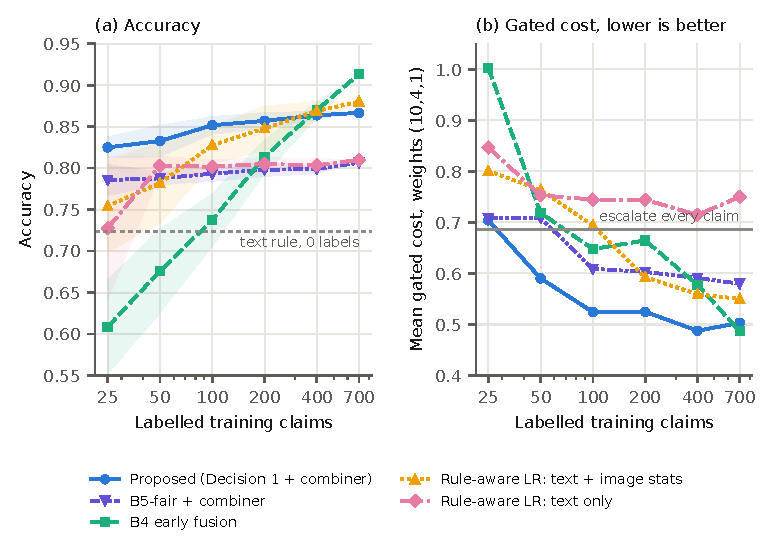
\includegraphics[width=\textwidth]{figures/fig_learning_curve.pdf}
\caption{Accuracy (a) and mean gated cost at weights $(10,4,1)$ (b) against the number of labelled training claims, on the 300 validation and test claims (ten stratified draws per size; shading in (a) is one standard deviation). Thresholds come from cross-fitted predictions inside each subsample. The rule-aware learners use features chosen with knowledge of the construction rules. B1 and B3 stay at or below 0.75 accuracy and are omitted.}\label{fig:lc}
\end{figure}

\paragraph{Efficiency.}
Decision~1 answers in a median of 0.80\,s (90th percentile 1.12\,s) with 1,087 input and no output tokens, about US\$0.11 per 1,000 claims; B5-fair takes 6.70\,s (10.10\,s) with 938 input and 335 output tokens, US\$1.96 (8.4 and 18 times more), and default B5 5.89\,s (8.18\,s) and US\$2.22. These are upper bounds, because the generative model still thought on 132 of 150 claims (243 tokens on average) despite a zero budget. Without thinking its median latency was 4.12\,s (about 5 times; 18 claims, not a random subset); default B5 is 7.4 times slower; answer tokens alone give 9.6 times the cost and input list prices alone 6.5 times. The advantage is thus about 5--8 times in speed and 6.5--18 times in cost, mostly list price, with runs eight hours apart; the absolute saving (about US\$1.85 per 1,000 claims and six seconds per claim) is small next to one human review.

\paragraph{Shortcut controls.}\label{sec:shortcuts}
Table~\ref{tab:short} applies the same checks to every method. The text rule equals the trained text model (0.747), and an image-quality detector separates escalations nearly as well as Decision~1's photograph check (AUC 0.932 against 0.957). On the matched subset, the text-based methods collapse, the image-only B3 scores highest (0.902 pooled, 0.909 on test), and the router and B4 tie at 0.805 (5 against 5 discordant claims); with 41 or 22 claims none of these differences is reliable. Degrading the clear photographs of the 103 test approvals and audits raised the share escalated from 28\% to 98\% (blur 100\%, low light 97\%, crop 97\%), and the photograph-clear answer fell from 0.51 to 0.19, near its 0.21 on true escalations. Without the 28 duplicated descriptions the router scores 0.844 and B4 0.926. Every method exploits construction rules, and the router's escalation route is largely a detector of the planted degradation.

\begin{table}[!htb]
\caption{Shortcut controls. Text rule: escalate theft or an unrecorded police report, audit a total loss, approve otherwise. A/R: the 103 test approvals and audits. Matched subset: approvals and audits reporting major damage with a recorded police status, pooled over validation and test (41 claims) and on test only (22).}\label{tab:short}
\footnotesize
\begin{tabular*}{\textwidth}{@{\extracolsep{\fill}}lcccc@{}}
\toprule
Method & Test acc. & A/R claims & Matched, val + test & Matched, test \\
\midrule
Text rule (no learning) & 0.747 & -- & 0.439 & -- \\
Proposed (tri-modal) & 0.853 & 0.825 & 0.805 & 0.682 \\
\quad no numbers & 0.880 & 0.845 & 0.902 & 0.818 \\
B1 text only & 0.747 & 0.757 & 0.341 & 0.318 \\
B3 image only & 0.727 & 0.631 & 0.902 & 0.909 \\
B4 early fusion & 0.913 & 0.883 & 0.805 & 0.773 \\
B5-fair + combiner & 0.813 & 0.777 & 0.585 & 0.545 \\
\botrule
\end{tabular*}
\end{table}

\paragraph{Ablations.}
In Table~\ref{tab:abl}, the routing question alone answers ``Fraud-Audit'' for almost every claim (0.427), so the combiner is essential and the checks carry most of the signal (0.867 alone). Removing the image costs 22 points and the text 15; the numbers add nothing (0.880 without them, $p=0.39$), as the labels never depend on amounts. Validation selected $\tau_s=0$, so the support term is unused. Cost differences between ablations are unreliable at 150 claims.

\begin{table}[!htb]
\caption{Ablations on the test split. Question ablations reuse the API responses and refit the combiner; modality ablations re-query Decision~1 without one input. Differences of a few points are within the noise of 150 claims.}\label{tab:abl}
\footnotesize
\begin{tabular*}{\textwidth}{@{\extracolsep{\fill}}lcccc@{}}
\toprule
Variant & Acc. & Macro-F1 & ECE & Cost \\
\midrule
Full method (tri-modal) & 0.853 & 0.852 & 0.042 & 0.473 \\
Routing question only, no combiner & 0.427 & 0.224 & 0.388 & 0.620 \\
Combiner on the routing question only & 0.647 & 0.571 & 0.091 & 0.620 \\
Combiner on the check questions only & 0.867 & 0.865 & 0.042 & 0.553 \\
Without $q_2$ / $q_3$ & 0.787 / 0.740 & 0.779 / 0.727 & 0.053 / 0.086 & 0.713 / 0.400 \\
Without $q_4$ / $q_5$ & 0.853 / 0.867 & 0.850 / 0.865 & 0.042 / 0.029 & 0.433 / 0.507 \\
Without the image / text & 0.633 / 0.707 & 0.592 / 0.673 & 0.103 / 0.089 & 0.660 / 0.660 \\
Without the numbers & 0.880 & 0.880 & 0.063 & 0.573 \\
Confidence-only gate ($\tau_s=0$) & 0.853 & 0.852 & 0.042 & 0.473 \\
\botrule
\end{tabular*}
\end{table}

\paragraph{Sensitivity to the cost model.}
Table~\ref{tab:cost} re-selects thresholds for each cost model. At weights of 5 to 10 times a review, both learned routers cost clearly less than escalating everything. At $(20,4,1)$ and $(20,8,1)$ the router's cross-validated advantage ($-0.120$ and $-0.105$) is unresolved and the fixed-split thresholds did not transfer; at $(50,10,1)$ every method escalates. Under handling cost no method is distinguishable from escalating everything: in H1 the router costs 0.975 against 1.000 ($-0.025$ $[-0.103,\,+0.053]$), settling 13\% of claims, and B4 1.010; in H2 the thresholds escalate almost everything. The router's advantage therefore rests on misrouting cost, in which correct audits and escalations are free, and the weights are assumptions.

\begin{table}[!htb]
\caption{Mean cost under each cost model, thresholds re-selected. Test: frozen gate, automated coverage in parentheses. CV: $5\times5$ cross-validation, confidence-only gate, straight-through share in parentheses; $^{*}$ corrected $p<0.05$ against escalating every claim.}\label{tab:cost}
\footnotesize
\begin{tabular*}{\textwidth}{@{\extracolsep{\fill}}lcccccc@{}}
\toprule
 & \multicolumn{3}{c}{Test ($n=150$)} & \multicolumn{3}{c}{Cross-validation} \\
\cmidrule(lr){2-4}\cmidrule(lr){5-7}
Cost model & Esc. all & Proposed & B4 & Esc. all & Proposed & B4 \\
\midrule
(5, 2, 1) & 0.687 & 0.307 (0.56) & 0.307 (0.69) & 0.686 & 0.296$^{*}$ (0.20) & 0.264$^{*}$ (0.25) \\
(10, 4, 1) & 0.687 & 0.473 (0.50) & 0.473 (0.63) & 0.686 & 0.440$^{*}$ (0.17) & 0.457$^{*}$ (0.21) \\
(20, 4, 1) & 0.687 & 0.633 (0.27) & 0.687 (0.00) & 0.686 & 0.566 (0.14) & 0.665 (0.10) \\
(20, 8, 1) & 0.687 & 0.713 (0.27) & 0.687 (0.00) & 0.686 & 0.581 (0.13) & 0.703 (0.08) \\
(50, 10, 1) & 0.687 & 0.733 (0.02) & 0.687 (0.00) & 0.686 & 0.734 (0.01) & 0.686 (0.00) \\
H1 (handling) & 1.000 & 1.033 (0.41) & 1.000 (0.00) & 1.000 & 0.975 (0.13) & 1.010 (0.02) \\
H2 (handling) & 1.000 & 1.000 (0.00) & 1.000 (0.00) & 1.000 & 1.013 (0.01) & 1.000 (0.00) \\
\botrule
\end{tabular*}
\end{table}

\paragraph{Error analysis and stability.}\label{sec:errors}
The most frequent error of both routers is a true audit predicted as an approval (9 of 22 errors for the router, 7 of 13 for B4; Fig.~\ref{fig:cm}). Every method misses the five test audits that pair a fraud-flagged minor claim with extensive damage, since the fraud flag is not an input, and B4's advantage concentrates in the police-status and total-loss subgroups decided by text rules. Re-sending the first 100 test claims eight hours later changed 6 of 53 automated decisions, all to escalation; only 10 responses were numerically identical and single answers moved by up to 0.197, and the re-test cannot detect changes over longer periods.

\begin{figure}[!htb]
\centering
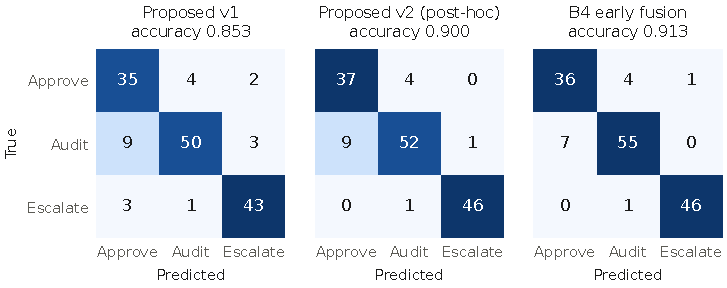
\includegraphics[width=0.85\textwidth]{figures/fig_confusion.pdf}
\caption{Test-set confusion matrices before gating, for the proposed method (v1), its post-hoc revision (v2) and early fusion (B4). Shading shows the row-normalised rate; numbers are counts.}\label{fig:cm}
\end{figure}

\paragraph{Post-hoc revision.}\label{sec:v2}
After the test evaluation, test errors showed that the routing question did not reflect the routing policy. A revised request (v2) states the routing rules, defines the options by visible evidence and adds police-status and theft questions. It raises zero-shot accuracy from 0.427 to 0.607 and, with the combiner, reaches 0.900 on test ($p=0.065$ against v1) and 0.897 in cross-validation (3.1 points above v1 $[0.5,\,5.7]$; $-1.1$ $[-3.4,\,+1.1]$ against B4). Test errors shaped it and its instruction restates the label rules, so v2 is exploratory.

\paragraph{Human oversight and limitations.}
People handle 80\% of claims at the default weights, and reviewer time and automation bias were not measured; the raw routing answer, almost always Fraud-Audit, should not be shown to reviewers, and an audit should be a triage flag, never an automated rejection. A degraded photograph alone triggers escalation, which would slow payment for claimants with poorer cameras, and identical requests can be routed differently, so each decision's scored response should be stored and audits should be contestable. Each decision sends the claimant's photograph and personal fields to an external service, which needs a lawful basis, retention terms and, for CarDD, the licensor's consent; every CarDD photograph in this study was sent to the Gemini API several times. Thresholds must be re-validated when the model changes, and automation should require a one-sided bound on the cost difference against escalate-all below zero. The study is limited by a small, constructed, rule-labelled benchmark with planted degradation, 150 test claims, a cost advantage that vanishes under handling cost, questions that carry the labelling rules, one proprietary model, efficiency ratios that are upper bounds, a 2026-only literature review, and analyses added after the test evaluation.

\section{Conclusion}\label{sec:conclusion}

This paper asked whether a closed-set decision model can route motor claims to automatic approval, fraud audit or human review from a photograph, a description and numerical fields, more cheaply than a generative model and with errors weighted by cost. The router sends all three inputs to Gemini Decision~1 in one request with a routing question and four yes/no checks, maps the answers to route probabilities with a 24-parameter combiner, and escalates uncertain claims through a validation-tuned confidence gate.

The answers are mixed. On the frozen test split the router reached 0.853 accuracy and trained early fusion 0.913, a difference the split could not resolve; in repeated cross-validation early fusion was 4.2 points more accurate at a cost the data cannot separate from the router's. When only misrouting is priced at moderate weights, both lowered cost against escalating every claim, but once every audit and escalation is charged as human work, neither did. With 25 labelled claims the router reached 0.825, against 0.754 for a learner given the labelling rules as features and 0.609 for early fusion; because the questions were written from those rules, most of that lead is rule knowledge in the prompt. Decision~1's answers were 5.2 points more accurate than a generative model's answers to the same questions, at about 5 to 8 times lower latency and 6.5 to 18 times lower cost, mostly owing to list prices and the generative model's residual thinking.

The controls qualify these results. A rule-only baseline matched the trained text model, an image-quality detector nearly matched the photograph check, and degrading a clear photograph made the router escalate almost every approval and audit. Part of every method's accuracy therefore reflects how the benchmark was built.

On this benchmark, a closed-set decision model asked policy-aligned questions is a fast, cheap source of routing features when few labels are available, but it does not replace a trained model when labels are plentiful, and its cost advantage depends on how human handling is priced. The study is limited by a small, rule-labelled benchmark, a proprietary model and thresholds that did not transfer at strict cost ratios. Future work should test the router on genuine claims labelled by claims handlers, decouple image quality from the label, compare other closed-set scorers such as option log-probabilities from open models, and measure reviewer workload and claimant outcomes in a supervised pilot.


\backmatter

\bmhead{Acknowledgements}
[To be completed by the authors, or removed if there are none.]

\section*{Declarations}
\begin{itemize}
\item \textbf{Funding:} [To be completed by the authors.]
\item \textbf{Competing interests:} [To be completed by the authors.]
\item \textbf{Ethics approval and consent to participate:} Not applicable. The study involves no human participants; it uses a public insurance-claims data set and the CarDD image set under its research licence.
\item \textbf{Data availability:} The benchmark pairs CarDD photographs~\cite{wang2023cardd}, which are available from their owners under a licence that forbids redistribution, with records from the public Auto Insurance Claims data set~\cite{kaggleclaims}. Neither the images nor the paired records are redistributed. The parsed model outputs and analysis results used in this paper are included in the code repository.
\item \textbf{Code availability:} Code, prompts, frozen configurations and evaluation scripts are available at \url{https://github.com/rajeshkadiyalaaa/Claim_detection_Mulimodel}.
\item \textbf{Author contributions:} [To be completed by the authors, for example using CRediT roles.]
\end{itemize}

\bibliography{references}

\end{document}
